%%%%%%%%%%%%%%%%%%%%%%%%%%%%%%%%%%%%%%%%%%%%%%%%%%%%%%%%%%%%%%%%%%%%%
%%%%%%%%%%%                   PROBLEM 2                   %%%%%%%%%%%
%%%%%%%%%%%%%%%%%%%%%%%%%%%%%%%%%%%%%%%%%%%%%%%%%%%%%%%%%%%%%%%%%%%%%

\section{پرسش دوم}
متودولوژی‌های چابک علیرغم تمام محاسن و امتیازاتی که برای توسعه به همراه دارند، ممکن است برای ایجاد هر نوع پروژه‌ی نرم افزاری مناسب نباشند!
گاهی اوقات لازم است برای موفقیت آمیز بودن پروژه از راه‌حل‌ها و پکیج‌های آماده یا روش‌های سنتی تولید نرم افزار استفاده شود یا راهکاری ترکیبی اتخاذ گردد.

واژه‌ی "فیلتر‌های تناسب"
\LTRfootnote{Suitability Filters}
به مجموعه‌ای از  پرسش‌ها و محک‌ها اطلاق می‌شود که به منظور بررسی مناسب بودن استفاده از یک متودولوژی چابک برای انجام یک پروژه‌ی نرم افزاری و با توجه به شرایط آن پروژه مطرح می‌شوند.

معمولا هر متودولوژی چابک برای  بررسی تناسب استفاده از آن برای پروژه‌ها چنین فیلتر‌هایی را ارائه می‌کند. این فیلتر‌ها معمولا ریسک‌های استفاده از متودولوژی مورد نظر را به توجه به شرایط پروژه، کارفرما و تیم آن گوشزد می‌شوند و معیاری برای تعیین مناسب بودن استفاده در اختیار قرار می‌دهند.


\begin{enumerate}[i]
\item \textbf{\lr{DSDM Suitability Filter}} \newline
مجموعه‌ای از پرسش‌های ساده‌ی و عموما به صورت بله/خیر است که ویژگی‌های پروژه، کارفرما و تیم را برای تصمیم در مورد استفاده از متودولوژی چابک DSDM مورد بررسی قرار می‌دهد.

از میان این پرسش‌ها می‌توان به این موارد اشاره کرد:

\begin{itemize}
\item 
آیا فلسفه‌ی توسعه‌ی چابک و مفاهیمی مانند بازه‌های زمانی
\LTRfootnote{Time boxes}
، مشارکت کاربر
\LTRfootnote{User involvement}
و توسعه‌ی مبتنی بر تکرار
\LTRfootnote{Iterative development}
قبل از شروع به کار مورد تایید است؟
\item
آیا اعطای قدرت تصمیم گیری به تیم‌های توسعه و تیم‌های کاربری مورد قبول است؟
\item
آیا مدیریت با حضور کاربران و در دسترس بودن آنها برای توسعه‌ی مشترک با آنها موافق است؟
\item
آیا تحویل تدریجی 
\LTRfootnote{Incremental delivery}
محصول مورد تایید و مقبول است؟
\item
آیا در دسترس بودن تیم توسعه برای مشتری و یا توسعه در مکان مشتری مورد قبول است؟
\item
آیا امکان حضور ثابت یک هسته‌ی تیمی از افراد برای حفظ پایه‌های اصلی پروژه و دانش آن به جای مستند سازی مفصل وجود دارد؟
\item
آیا تیم توسعه تیمی قوی و با مهارت‌‌های ارتباطی خوب است؟
\item
 آیا تیم توسعه تیمی کوچک و متشکل از تعداد کمی از افراد است؟
\item
آیا مبنای اعتماد و تعامل به جای مذاکره و چانه زنی مورد قبول است؟
\item
آیا تکنولوژی توسعه از ویژگی‌هایی مانند تحویل تدریجی، مدلسازی سریع و refactoring پشتیبانی می‌کند؟
 
\end{itemize}

پاسخ‌های مثبت و منفی به هر یک از سوالات می‌تواند دید خوبی را نسبت به مناسب بودن استفاده از متودولوژی چابک در اختیار قرار دهد. منفی بودن پاسخ تعداد معدودی از سوالات لزوما نشانه‌ی نامناسب بودن استفاده از توسعه‌ی چابک نیست ولی احتمال بروز چالش‌هایی را در صورت استفاده گوشزد می‌کند. منفی بودن پاسخ تعداد زیادی از سوالات احتمالا نشانه‌ی این است که بهتر است از متودولوژی چابک استفاده نشود، زیرا چالش‌های پیش رو بسیار زیاد خواهند بود!

\item \textbf{\lr{Alistair Cockburn’s Criticality and Team Size Factors}} \newline

این فاکتور‌ها مخصوص خانواده‌ی Crystal از متودولوژی‌های توسعه‌ی چابک نرم‌افزار است که بر اساس تناسب پروژه‌ی نرم افزاری به اظهار نظر در مورد آن می‌پردازد.

این فاکتور‌ها متودولوژی‌های Crystal و پروه‌های متناسب آنها را بر اساس میزان حساسیت پروژه‌ی نرم افزاری و تعداد اعضای تیم توسعه دسته بندی می‌کند:

\begin{center}
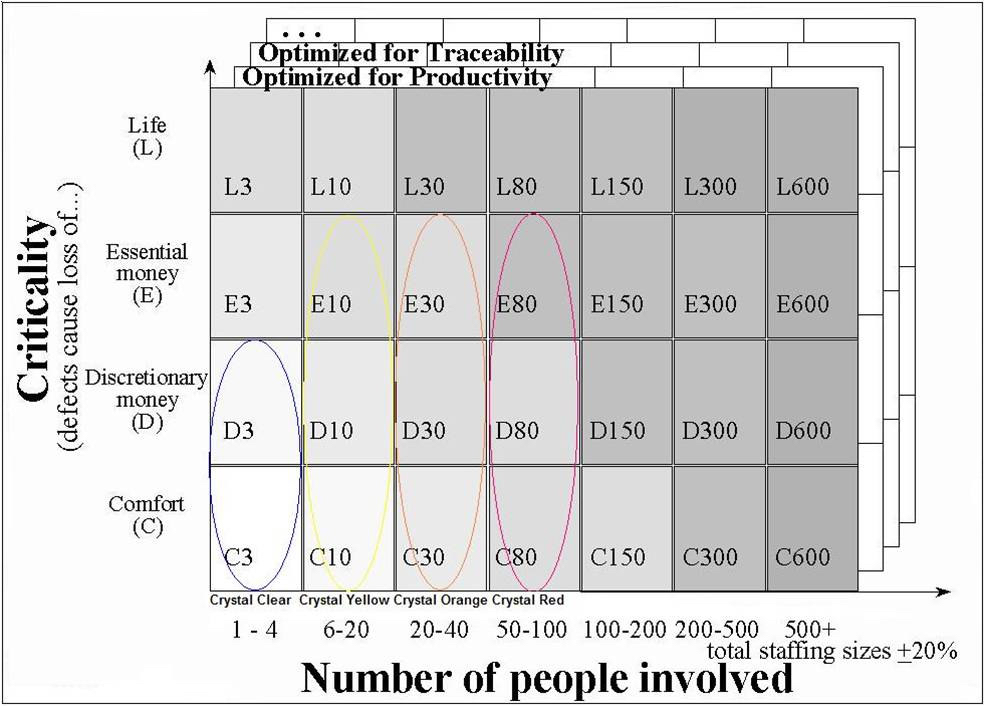
\includegraphics[width=0.8\textwidth]{images/Agile-Crystal}

منبع تصویر:
LeadingAnswers
\LTRfootnote{\url{http://leadinganswers.typepad.com/leading_answers/files/agile_suitability_filters.pdf}}
\end{center}


محور افقی مبین تعداد اعضای تیم توسعه و محور عمودی بیانگر حساسیت سیستم است (معیاری از خسارتی که در صورت خرابی سیستم وارد خواهد شد: هیچ - مالی اندک - مالی شدید - جانی).

قابل مشاهده است که متودولوژی \lr{Crystal Clear} برای تیم‌های کوچک تا ۴ نفره و برای پروژه‌های تا سطح ریسک مالی اندک مناسب است و متودولوژی‌های سنگین تر دیگر خانواده‌ی Crystal برای تیم‌های تا حداکثر ۱۰۰ نفر و تا سطح خسارت مالی شدید مناسب اند.

متودولوژی‌های چابک برای تیم‌های کوچک بسیار مناسب عمل می‌کنند. استفاده از این متودولوژی‌ها برای تیم‌های بزرگ نیز می‌تواند مناسب باشد اما نیازمند تجربه فراوان و مدیریت درست است.
\cite{agile-suitability-filters}

\end{enumerate}